\section{Hall-sensor}

The velocity calculation is done trough the Hall sensors. There are four magnets on the gear at approximatly a quarter of a turn of distance each. One way of getting the speed is by calculating the time between each outputs and the distance traveled during that time. A plot of the speed can be seen on \figref{unfilteredHall}.

\begin{figure}[H]
	\centering
	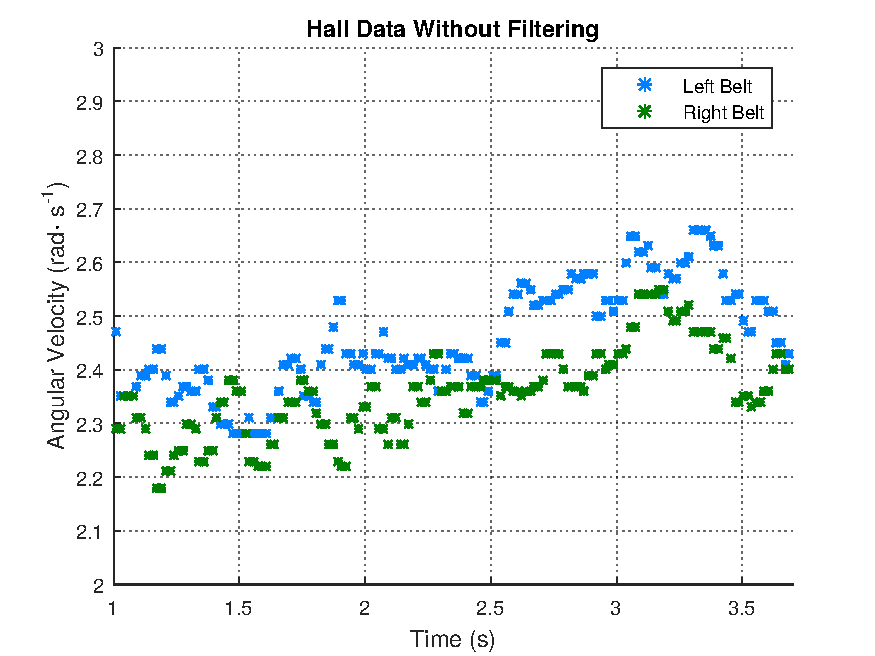
\includegraphics[scale=0.9]{figures/unfilteredHall.pdf}
	\caption{Plot of an unfiltered measurement by the Hall Sensors at full speed}
	\label{unfilteredHall}
\end{figure}


This is a plot of the speed, with unaccurate measurement because of the uneven placement of the magnets, with a calculation of the time between each magnets.\\


The new approach is to get the time the wheel take to make a full turn, to have the exact time and distance of a rotation. The speed will be calculated from a full turn every magnets, compared to the last time it was registered, four outputs before. A plot of the measurements can be seen on \figref{filteredHall}.

\begin{figure}[H]
	\centering
	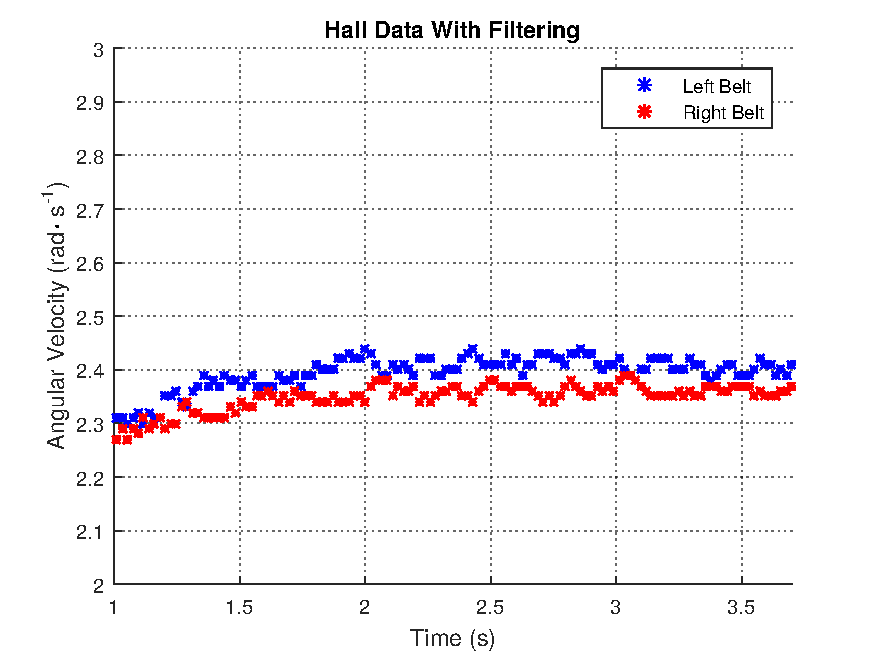
\includegraphics[scale=0.9]{figures/filteredHall.pdf}
	\caption{Plot of an filtered measurement by the Hall Sensors at full speed}
	\label{filteredHall}
\end{figure}

The difference between the two plots is that at constant speed, the time measured at each outputs is uneven on \figref{unfilteredHall}, and even in \figref{filteredHall}. A flowchart of the implementation of the functions of the Hall Sensors can be seen on \figref{hallFlowchart}.

\begin{figure}[H]
	\centering
	\includegraphics[scale=0.9]{figures/hallFlowchart.pdf}
	\caption{Flowchart of the two main functions \textit{tSpeed} and \textit{getSpeed} of the Hall Sensors implementation}
	\label{hallFlowchart}
\end{figure}

This flowchart explains the way of getting the time at each outputs. The Hall Sensors use the timers 4 and 5 to register the time of the output. The first function \textit{tSpeed} describes the storing of the two timers values in the registers, the second is a subfunction of the first one, and the last function \textit{getSpeed} is the calculation of the speed from the raw data of a variable in the function \textit{tSpeed}.\\

\subsubsection{FIR Filter}

Using the four magnets of the wheel and recording the time values through the timers involve using a  FIR Filter(Finite Impulse Response Filter). An overview of the filter can be seen on \figref{FIRFilter}.


\begin{figure}[H]
	\centering
	%\includegraphics[scale=0.9]{figures/FIRFilter.pdf}
	\caption{Overview of an FIR Filter}
	\label{FIRFilter}
\end{figure}